% file to contain information on examples
%==============================================================================
\chapter{Examples - WIP}
Examples are located in the \verb|0-examples| folder and are designed to be run in batch mode.
This means that each example copies any required system, model, or modulation file to the main PST directory before running.
Typically, each example folder contains a \verb|.m| file that starts with \verb|run_| that can be used to run the example.
As example cases are located on a github repository, relative file paths are used so that examples can be run without much difficulty from various different machines.
While most examples can be run in multiple versions of PST, some functionality can only be found in specific versions.


\section{Example Operation Overview}

\noindent The general structure of created examples tend to reflect the following:
\begin{enumerate}
\itemsep 0em
\item Clear all variables, close all figures, and clear the command window.
\item Define which version of PST to use.
\item Create a relative path to the root directory of chosen PST version.
\item Copy any system, model, or modulation file to the PST root directory.
\item Set live plotting flag.
\item Run \verb|s_simu|.
\item Save output data.
\item Restore any model, or modulation file to original state.
\item Create data plots.
\end{enumerate}

A high level flow chart of the \verb|s_simu| script is presented in Appendix \ref{sec: simu BD}.
It should be noted that in \verb|s_simu|, an optional \verb|g.sys.DEBUG| flag may be set to 1 to display more output to the console.
%=================================================================
\pagebreak
\section{Standard Faulting (hiskens)}
Standard PST simulations involve some kind of fault defined in the \verb|sw_con| array.
This example (located in the \verb|hiskens| folder) is included to showcase some simple differences between PST versions using a standard test case.
System data for this example comes from a report by Ian Hiskens \cite{hiskens2013} which summarized a study of an IEEE 10 generator, 39 bus system.
Ryan Elliott at Sandia National Labs recreated the system in a PST format and provided the data file for this project.
A one-line diagram of the system is shown in Figure \ref{fig: hiskens oneline}.

\begin{figure}[H]
	\centering
	\footnotesize
	\includegraphics[width=.85\linewidth]{figures/hiskens/hiskensOneline}
	\caption{IEEE 39 bus network.}
	\label{fig: hiskens oneline}
\end{figure}%\vspace{-1 em}

The simulated event was a 0.1 second three-phase fault with no loss of line between bus 2 and 3.
The \verb|run_datane_hiskens.m| file can be used to run the simulation.
Figure \ref{fig: hiskens results} shows the resulting fault bus voltage magnitude and system generator speeds.

\begin{figure}[H]
	\centering
	\footnotesize
	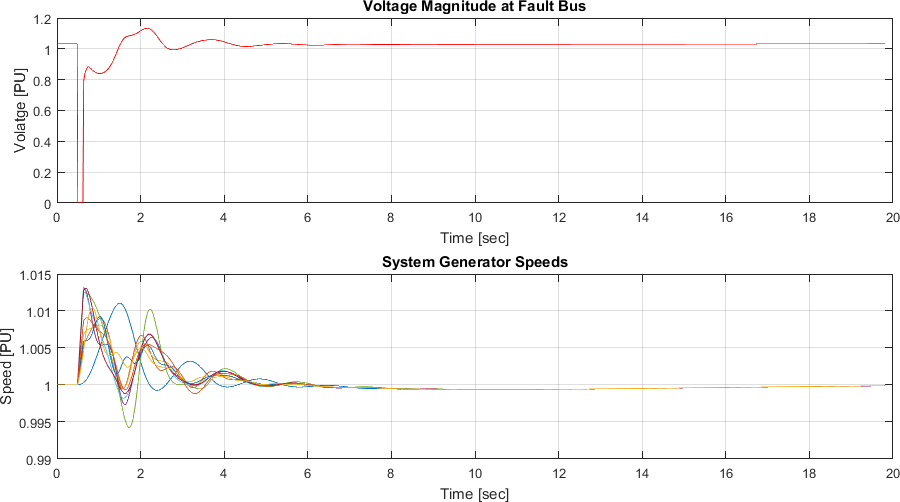
\includegraphics[width=\linewidth]{figures/hiskens/hiskensResults}
	\caption{Hiskens Example Fault Bus Voltage and Generator Speeds.}
	\label{fig: hiskens results}
\end{figure}%\vspace{-1 em}

All PST versions (when using the same models) provide the same results, but there are differences in simulation speed and data output.
Table \ref{tab: hiskens} shows that the PST 4 simulation was roughly twice as fast as PST version 2 or 3, saved less data, and left fewer variables in the MATLAB workspace post simulation.
These improvements are likely due to the restructuring of global variables and code to remove any `all zero` data from being saved.\\

% table data for hiskens fault comparison 


\begin{table}[H]
%\resizebox{\linewidth}{!}{ % Use to resize large tables
\singlespacing
	\begin{tabular}{@{} L{1.75cm} 
	R{2cm} R{2cm}  R{2cm} @{}} 	
		\toprule % @ signs to remove extra L R space
		\footnotesize % this will affect the table font (makse it 10pt)
		\raggedright % for non justified table text
						
										
										
		PST Version	&	Simulation Time [seconds]	&	Resulting Workspace Variables	&	Saved Data Size [KB]	\\ \midrule	
		2.3	&	16.56	&	206	&	7,549	\\	
		3.1	&	16.70	&	210	&	7,548	\\	
		SETO	&	8.42	&	24	&	3,965	\\	
		4	&	7.96	&	6	&	3,974	\\	\bottomrule

													
	\end{tabular}

	\caption{PST Version Comparisons of Hiskens Example.}
	\label{tab: hiskens}
%	}%end resize box
\end{table}


%=====================================================================
\section{Modulation Examples} \label{sec: modExamples}
PST provides numerous ways to input a defined modulation signal into a variety of models.
The following list of example folder names work in all versions of PST and typically create linear/non-linear comparison plots.
While the examples themselves do not reflect any particular scenario, the provided code may be useful to create a particular scenario.

\begin{itemize}
\item \verb|lmod| - Replaces the \verb|ml_sig| file to modulate real load power.
\item \verb|mexc| - Replaces the \verb|mexc_sig| file to modulate the exciter reference signal.
\item \verb|mtg_sig| - Replaces the \verb|mtg_sig| file to modulate the governor $P_{ref}$ reference signal.
\item \verb|pm_sig| - Replaces the \verb|mpm_sig| file to modulate a machines mechanical power.
\item \verb|rlmod| - Replaces the \verb|rml_sig| file to modulate a load's reactive power.
\item \verb|SVC| - Replaces the \verb|msvc_sig| file to modulate an SVC's output value.
\item \verb|TCSC| - Replaces the \verb|mtcsc_sig| file to modulate an TCSC's output value.
\end{itemize}

\noindent It should be noted that modulation files for PST 2 and 3 assume input to function is ($t, k$), i.e. full time vector and data index, while PST 4 only requires the data index $k$.

%=====================================================================
% all current examples
\pagebreak
\section{Lightly Introduced Examples}
These examples exist on github, but don't necessarily require a much more than a casual mention.
\subsection{DC - WIP}
All versions - 

non-linear simulation seems to work

linear analysis doesn't seem to work correctly - user error?

\subsection{exciterBatchTests - WIP}
PST 4 only - used to compare all 4 exciter models linear/non-linear response to load step

Was useful in ensuring exciter models were cast to globals correctly

\subsection{inductive - WIP}
meant to verify functionality of inductive generators and loads (motors)

Multiple cases run from example script: fault example and load pulse with linear/non-linear comparison.
Works in all versions.

\subsection{tg - WIP}
Examples of a load step with and without governor action

%=====================================================================
\pagebreak
Examples from 0-examples folder are listed below - last bit of User manual work will be to `thin the herd', insert previous results, confirm working, and provide minor details about content


\section{AGC - WIP}
PST 4 only

\subsection{run\_AGC - WIP}
- 2 area kundur with optional integration methods = load step - 120 second recovery.


% can't include for some reason... must be input
\pagebreak
\subsection{run\_AGC\_mod - WIP}
Sloppily copied from: \verb|200821-AGCicAdjTest|

uses Interchange modulation signal as perturbance

\textbf{AGC Modulation Test (Interchange adjustment) } \ \\

\begin{minipage}{0.5\linewidth}
\begin{itemize}
\raggedright
\item Event: When $t=5$ Area 2 increases its scheduled interchange by 0.2 PU.\\
Area 1 interchange is adjusted by -0.2 PU to keep system in balance.\\
Area 2 increases generation while Area 1 reduces generation.

\item Each area has non-conditional AGC set to act every 15 seconds and is forced to act by \verb|mAGC_sig| when the interchange adjustment first takes place.

%\item ODE solver tolerances:
%\subitem Relative: 1e-5
%\subitem Absolute: 1e-7
\end{itemize}
\vfill
\end{minipage}\hspace{2em}% 
\begin{minipage}{0.4\linewidth}
\centering
\includegraphics[width=\linewidth]{examples/agcMod/sysOneLineAreas}
\end{minipage}% 


\textbf{Result Summary:}
\begin{itemize}
\item Interchange adjustment seems to work correctly and is accounted for in AGC calculations.
\item The use of \verb|mAGC_sig| was tested as working using FTS or VTS.
\end{itemize}

\begin{minipage}{.5\linewidth}

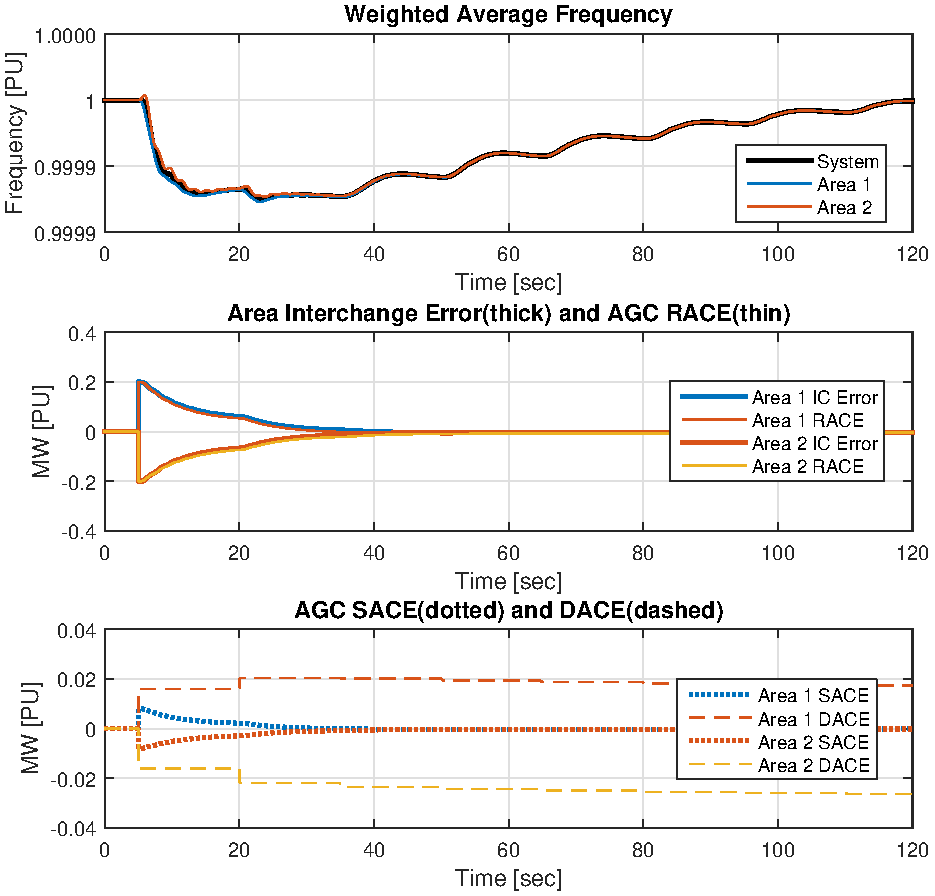
\includegraphics[width=\linewidth]{examples/agcMod/agcSigs}
\end{minipage}%
\begin{minipage}{.5\linewidth}

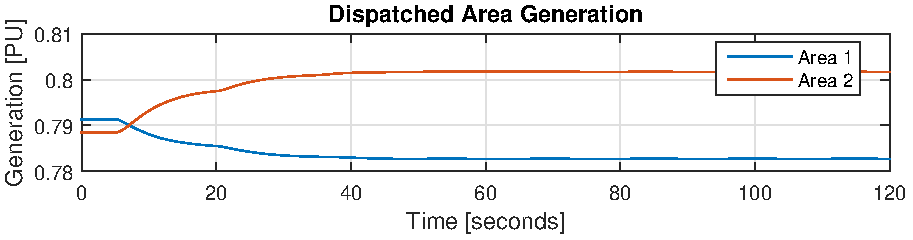
\includegraphics[width=\linewidth]{examples/agcMod/areaGen}

\vspace{1em}
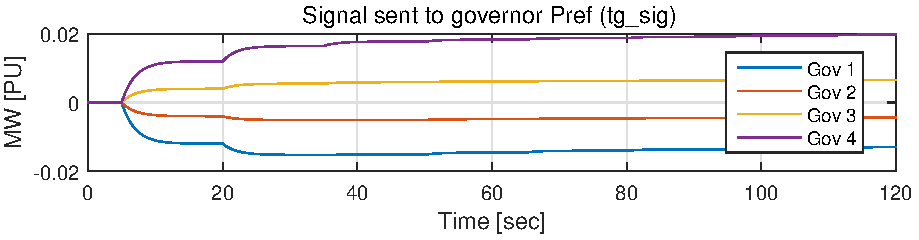
\includegraphics[width=\linewidth]{examples/agcMod/tgSigs}

\vspace{1em}
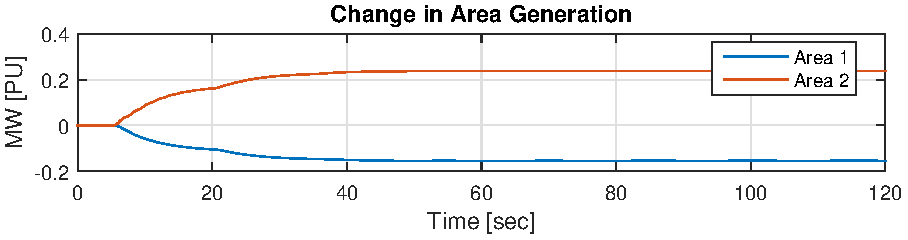
\includegraphics[width=\linewidth]{examples/agcMod/changeGen}
\end{minipage}

\textbf{Why this might matter: }
An extended term simulation may required the adjustment of scheduled interchange to achieve system recovery.
Specifically, if an area realizes that their available reserves become lower than was originally allocated for, a resolution may be to import more power from another area.
This added functionality will allow custom logic to handle such a scenario.

\pagebreak
\textbf{MATLAB modulation code} 
The \verb|mAGC_sig| file that adjusts the interchange and forces AGC action is shown below.


\begin{minted}[
		frame=lines,
		framesep=2mm,
		baselinestretch=1.2,
		bgcolor=gray!13,
		fontsize=\footnotesize,
		linenos,
		breaklines
		]{MATLAB}
function mAGC_sig(k)
% Syntax: mAGC_sig(k)
% input k is current data index
% 09:46 08/21/20
% place to define modulation signal for AGC operation

global g

%{
    Scenario:
Area 1 is exporting generation to Area 2 (Interchange value Positive)
Area 2 is importing power from Area 1 (Interchange value is Negative

Area 2 increases scheduled interchage, which reduces its scheduled import and causes area 2 to increase generation.
Area 1 decreases scheduled interchange to balance area 2 action.
As area 1 is exporting, the negative valued icAdj will reduce the generation in the area.

%}
persistent ForceDisptach

if g.sys.t(k) >= 5
    % adjust iterchange 
    g.area.area(2).icAdj(k) = 0.2;
    g.area.area(1).icAdj(k) = -0.2;
    
    % force AGC disptatch when interchange adjustment first applied
    if ForceDisptach
        g.agc.agc(1).nextActionTime = g.sys.t(k);
        g.agc.agc(2).nextActionTime = g.sys.t(k);
        ForceDisptach = 0;
    end
    
else
    g.area.area(2).icAdj(k) = 0;
    g.area.area(1).icAdj(k) = 0;
    ForceDisptach = 1;
end
end
\end{minted}




%=======================================================================
\pagebreak
\section{extendedTerm - WIP}
% copied from  200806-ExtendedVersionComp

\textbf{Scenario} (sloppily copied from 200806-ExtendedVersionComp)
 \begin{center}
\begin{minipage}{.47\linewidth}
\centering
\includegraphics[width=\linewidth]{examples/extendedTerm/sysOneLineAreas}
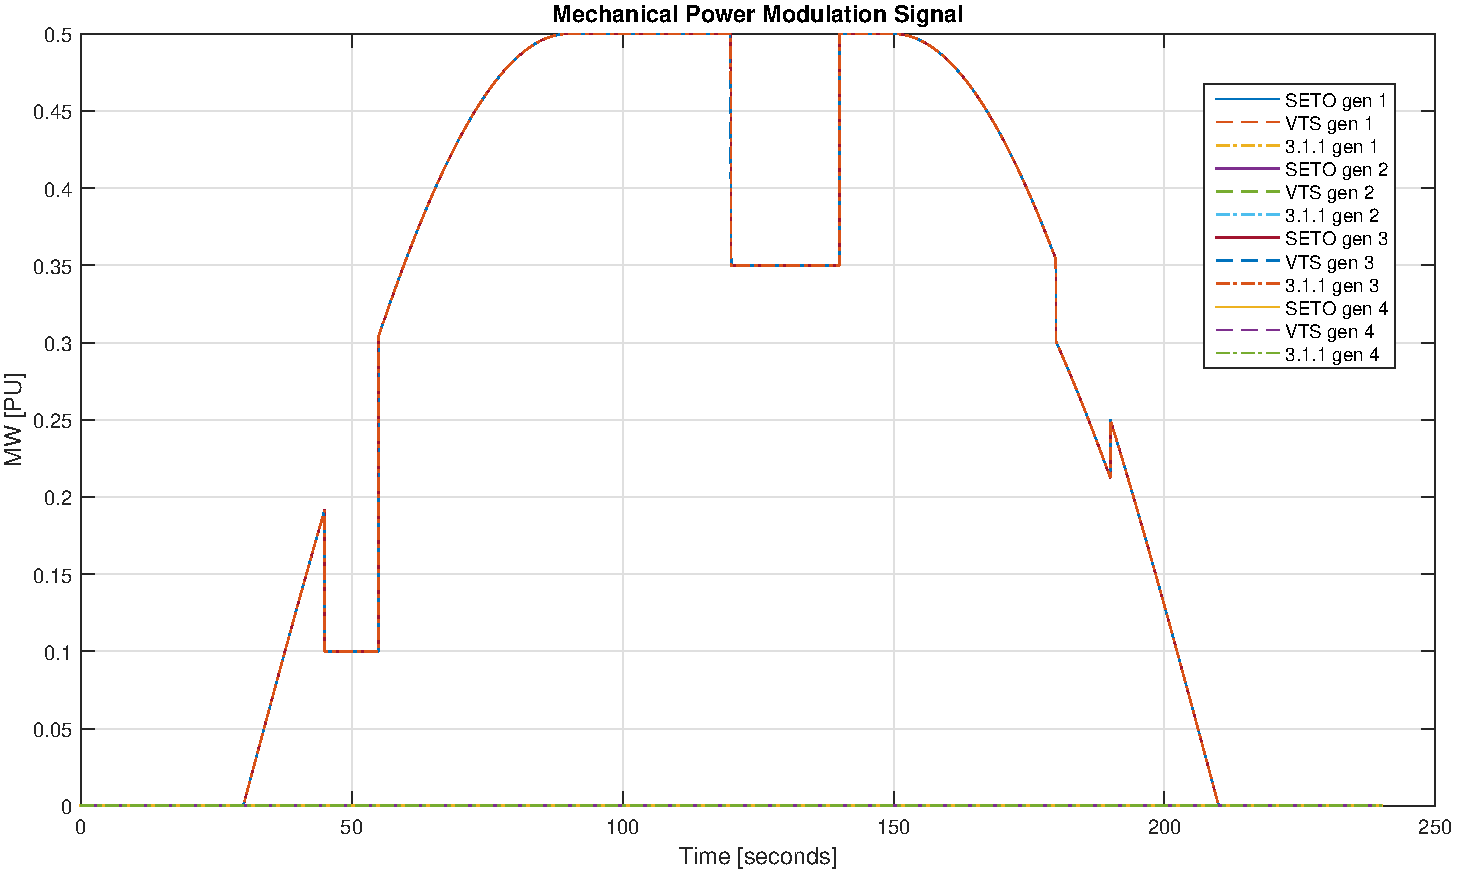
\includegraphics[width=.8\linewidth]{examples/extendedTerm/verPmSig}
\end{minipage} %
\begin{minipage}{.47\linewidth}
\begin{itemize}
\footnotesize
\itemsep 0em
\item Kundur  4 machine system packaged with PST
\item Constant Z load model
\item System has governors, exciters, and PSS.
\item Governor of generator being perturbed by pm\_sig removed
\item Perturbance was meant to mimic a solar ramp with various situations of cloud cover:\\
(larger plot of pm\_sig on Page 6)
\begin{Verbatim}[fontsize=\scriptsize]
% time [seconds]
% 0-30      - no action
% 30-90     - ramp up 0.5 PU (50 MW)
% 90-150    - hold peak
% 150-210   - ramp down 0.5 PU (50 MW)
% 210-240   - no action

% cloud cover events
% 45-55 - 20% max gen (generation of 0.1 PU)
% 120-140 - 30% cover (generation reduction to 70%)
% 180-190 - 15% cover (generation reduction to 85%)
\end{Verbatim}
\end{itemize}
\end{minipage}

\end{center}

\textbf{Summary} 
\begin{enumerate}
\itemsep 0 em
\item The PST 4 is 3.65 times faster than PST 3.1
\item Using variable time steps allows for a speed up of 14.84 over PST 3.1.
\item Results from all simulations are very similar.
\item Without creating an explicit time block at the beginning of an event, VTS events may not occur at the exact time they are programmed.
\item VTS reduces logged data size by $\approx$4 times.
\end{enumerate}


\begin{table}[!ht]
\resizebox{\linewidth}{!}{

	\begin{tabular}{@{} L{1.75cm} 
	R{2cm} R{2cm}  R{2cm} R{1.5cm} R{0.75cm} R{0.75cm} R{1.5cm} R{2cm} R{2cm}@{}} 	
		\toprule % @ signs to remove extra L R space
		\footnotesize % this will affect the table font (makse it 10pt)
		\raggedright % for non justified table text

	&	\multicolumn{3}{c}{Step Size [seconds]}					&		&	\multicolumn{2}{c}{Solutions Per Step}			&		&		&		\\	
\shortstack{PST\\Version}	&	Max.	&	Min.	&	Ave.	&	Total Steps	&	Ave.	&	Max.	&	Total Slns.	&	Sim. Time	&	Speed Up	\\ \midrule	
3.1	&	4.00E-03	&	4.00E-03	&	4.00E-03	&	59,975	&	2	&	2	&	119,950	&	916.24	&	1.00	\\	
4.0	&	4.00E-03	&	4.00E-03	&	4.00E-03	&	59,975	&	2	&	2	&	119,950	&	250.82	&	3.65	\\	
VTS	&	2.32E+01	&	2.68E-04	&	2.58E-02	&	9,315	&	2	&	97	&	17,006	&	61.73	&	14.84	\\	
																				\bottomrule
	\end{tabular}
	}%end resize box
	



\end{table}


\pagebreak
% fixed: 8749 steps i.e., 17498 network solutions 

%>> compareVTSandFTS
%VTS time: 15.8579
%fixed time: 57.4479
 

\textbf{Plotted Results - Step Size / Number of Solutions Comparison} \ \\
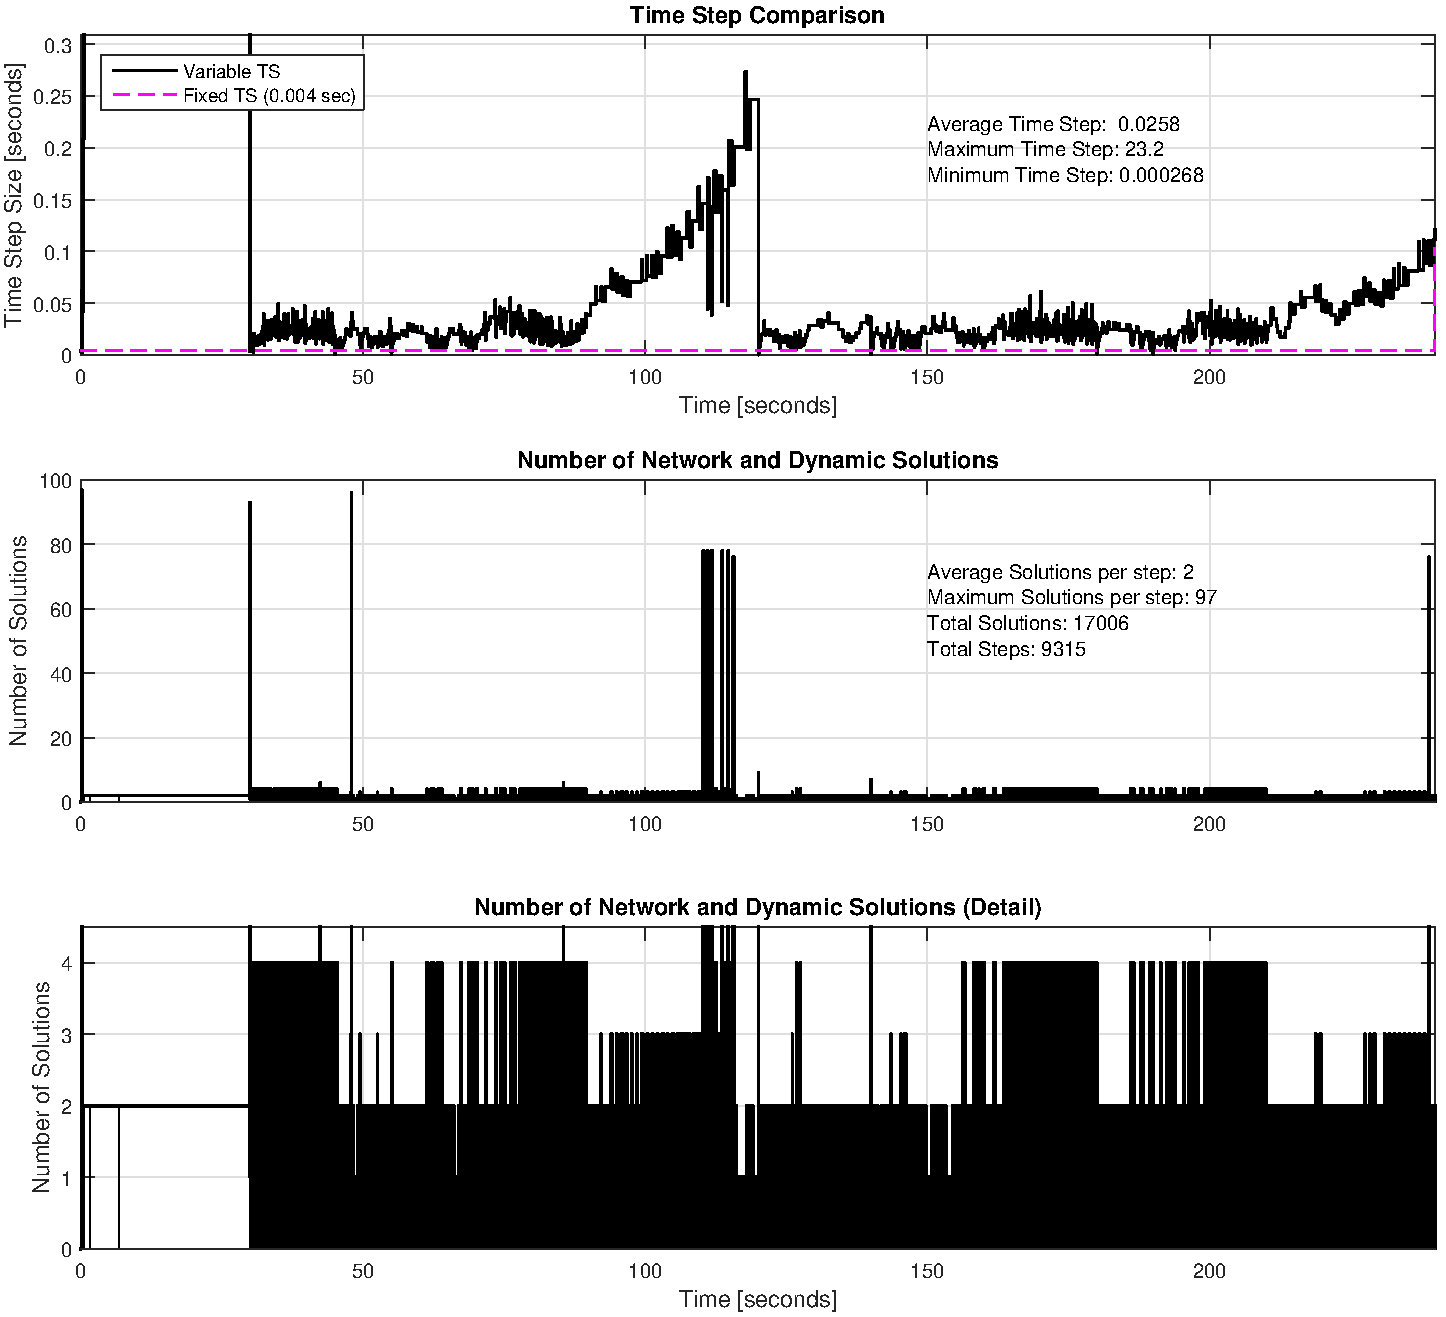
\includegraphics[width=\linewidth]{examples/extendedTerm/verSteps}

NOTE: Initial time steps before t=30 are much larger than the other time steps (multiple seconds) and are plotted off the axis.

\pagebreak
\textbf{Plotted Results - Various Comparisons} \ \\
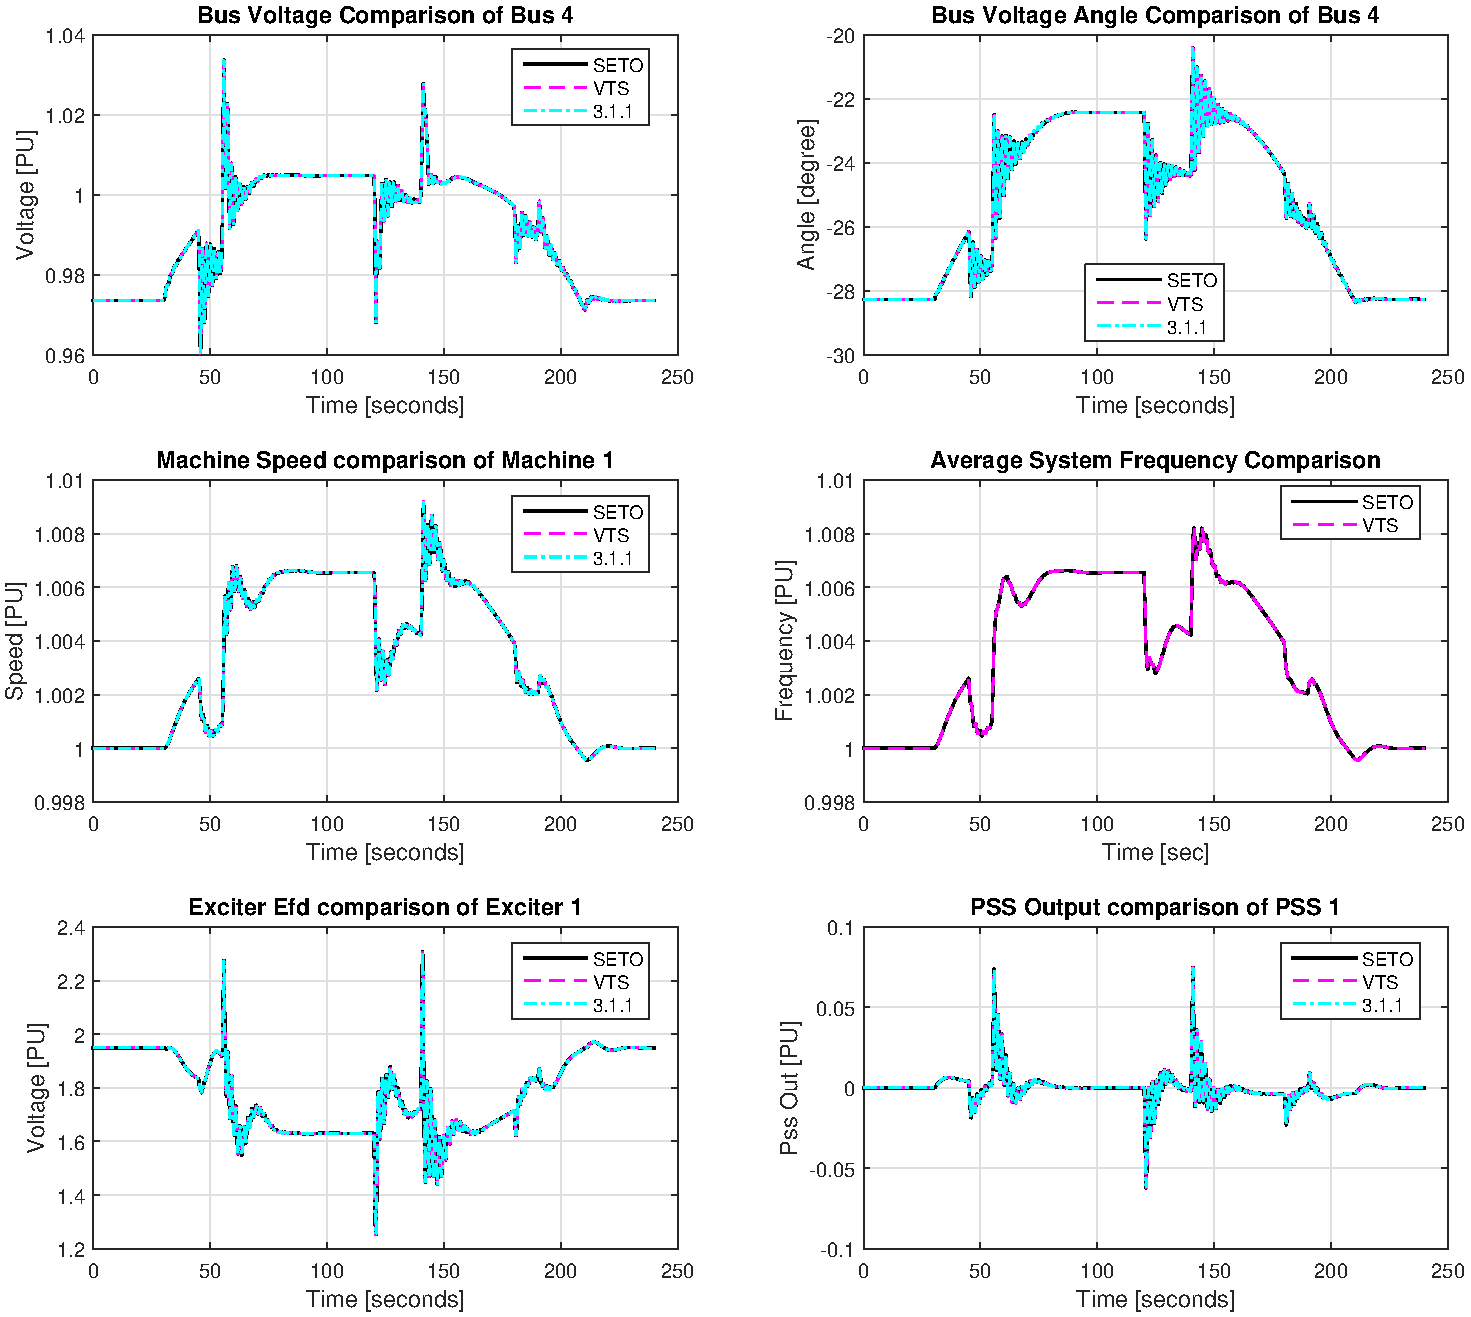
\includegraphics[width=\linewidth]{examples/extendedTerm/verComp}

NOTE: 3.1 does not calculate average system frequency.

\pagebreak
\textbf{Plotted Results - Various Comparisons - Detail 1} \ \\
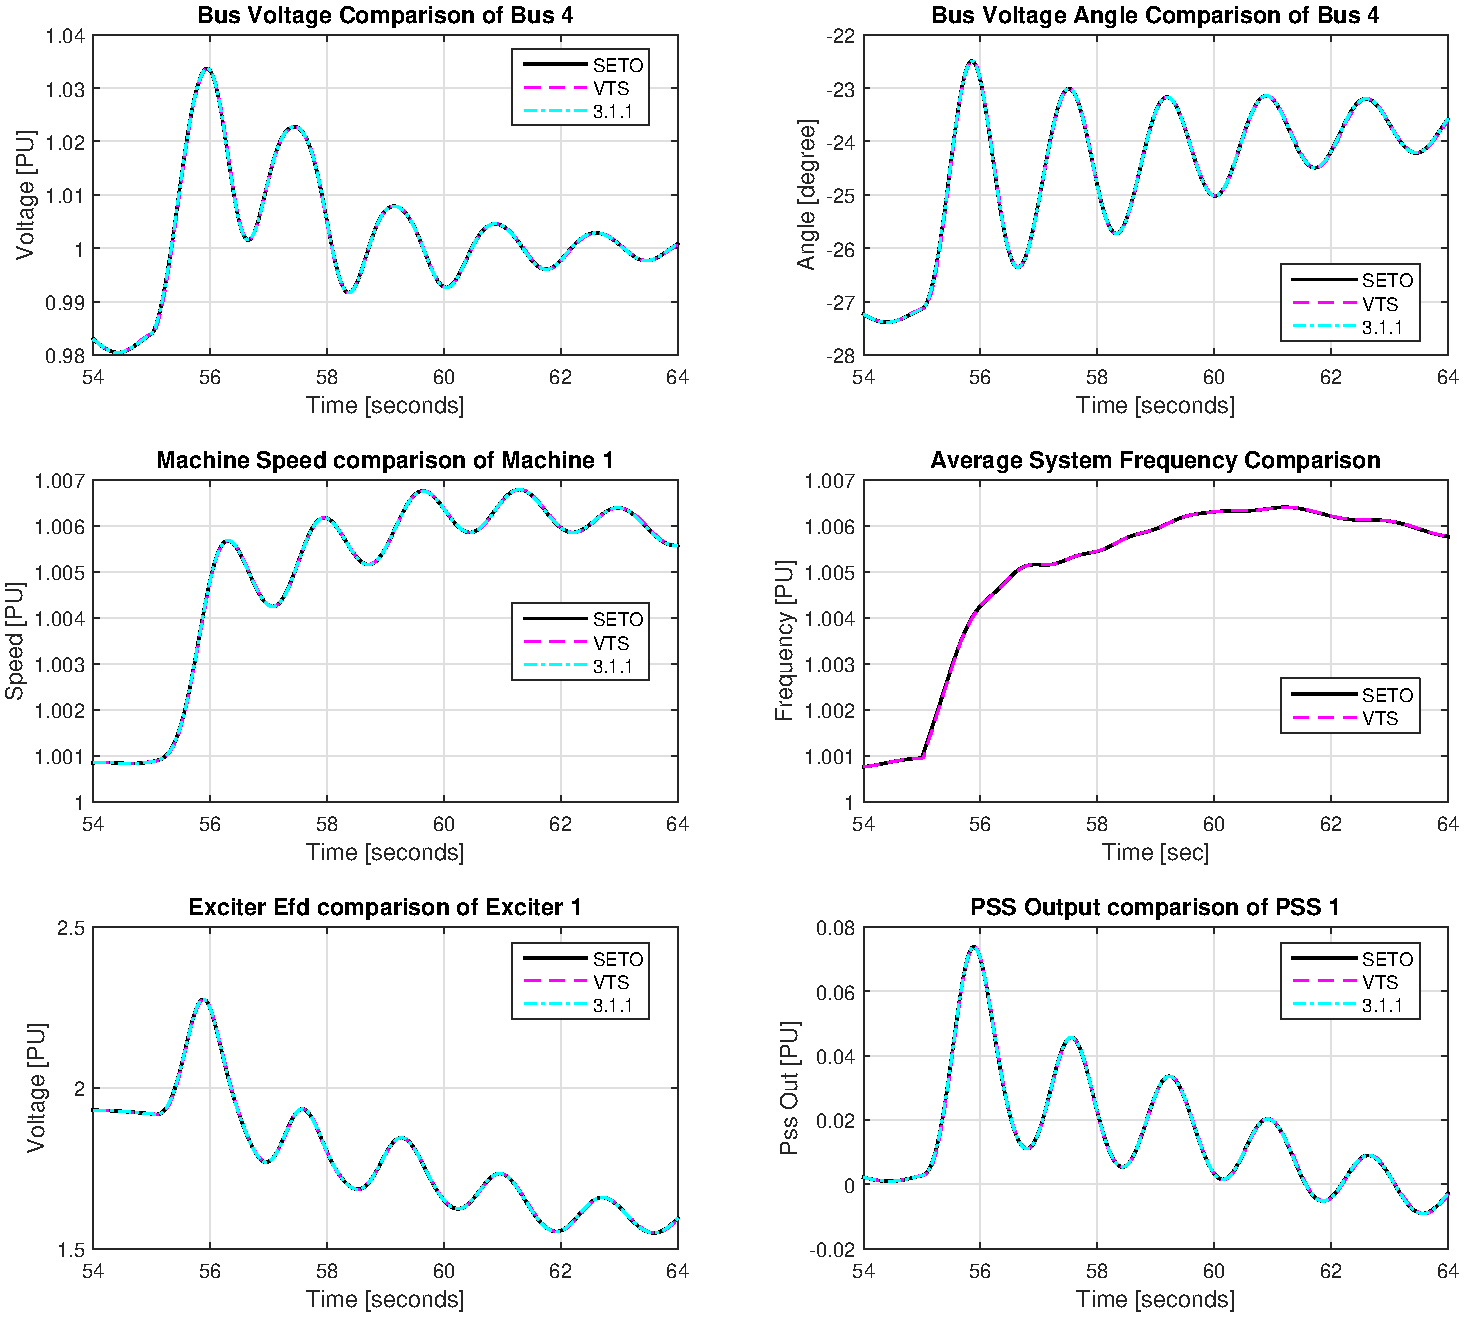
\includegraphics[width=\linewidth]{examples/extendedTerm/verCompDetail1}

NOTE: 3.1 does not calculate average system frequency.

\pagebreak
\textbf{Plotted Results - Various Comparisons - Detail 2} \ \\
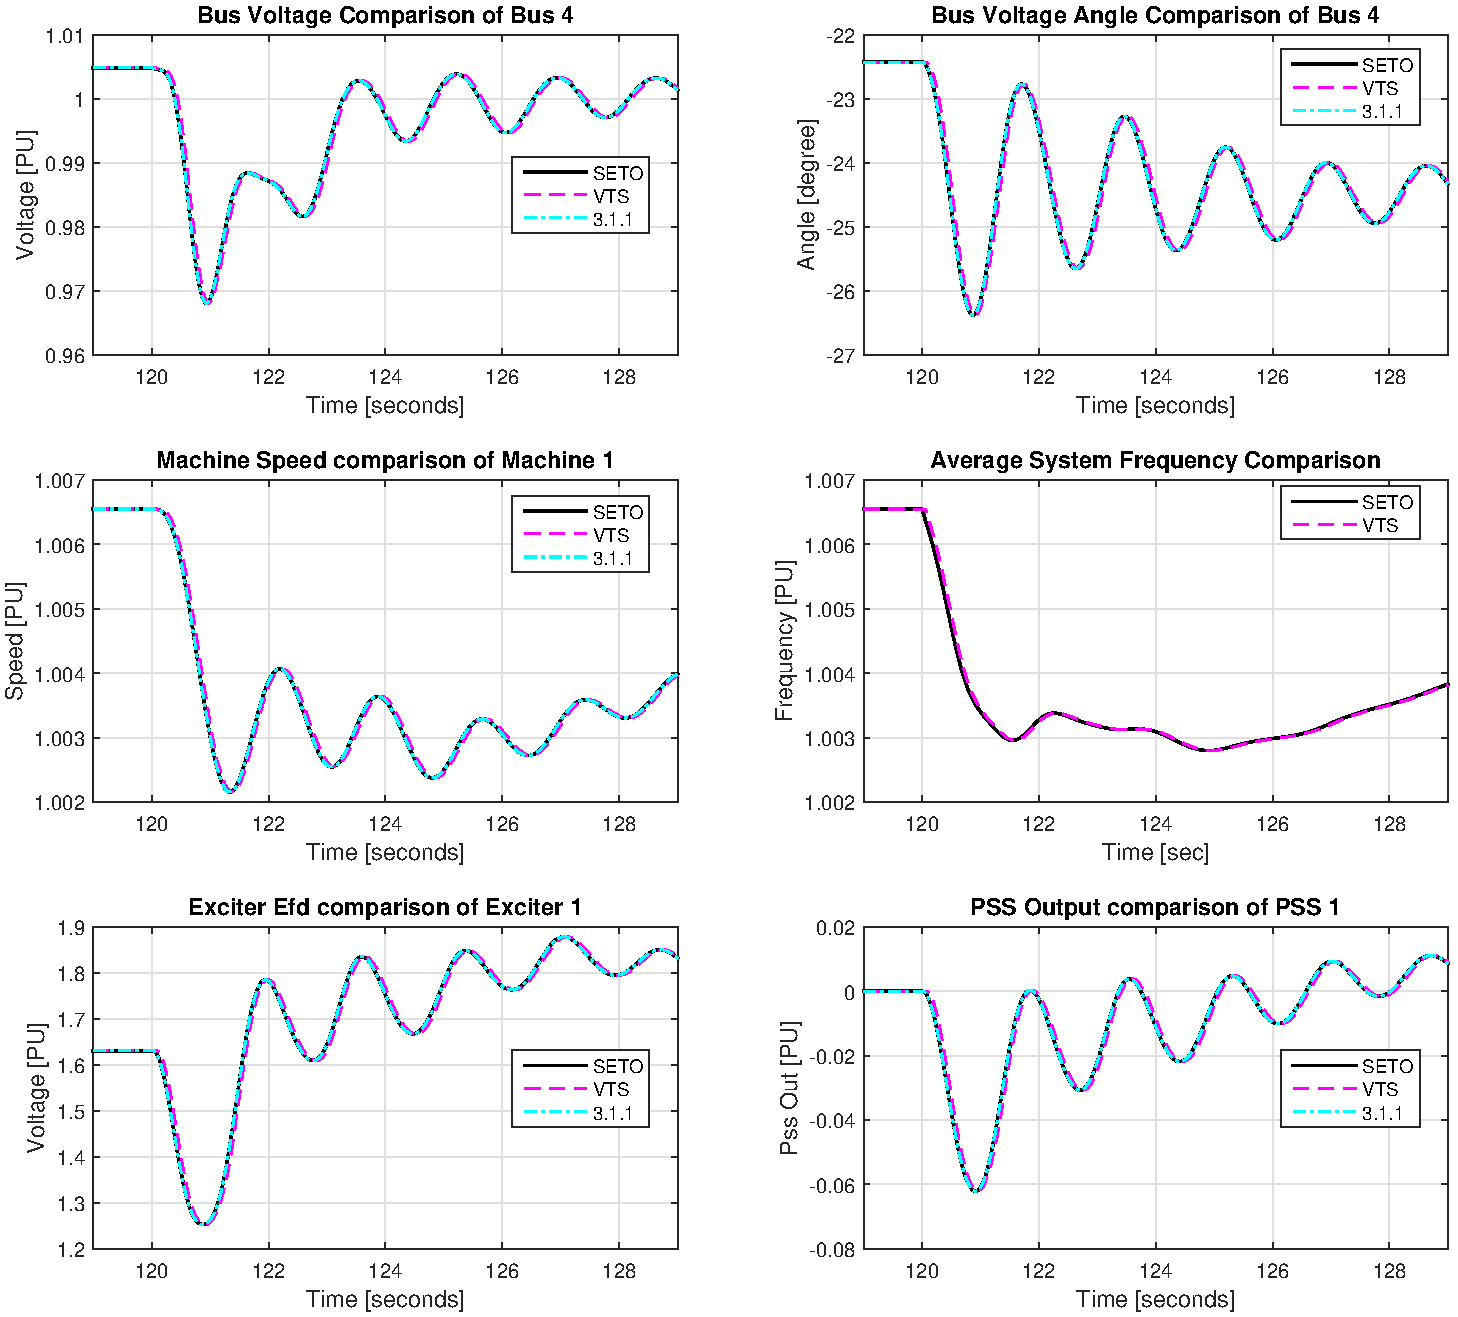
\includegraphics[width=\linewidth]{examples/extendedTerm/verCompDetail2}

NOTE: 3.1 does not calculate average system frequency.

VTS events may not occur at exact specified time due to the nature of variable time steps.

Breaks in the \verb|sw_con| can be created to account for this, however, the variance in time is often relatively small.


\pagebreak
\textbf{Plotted Results - Modulation Signal} \ \\
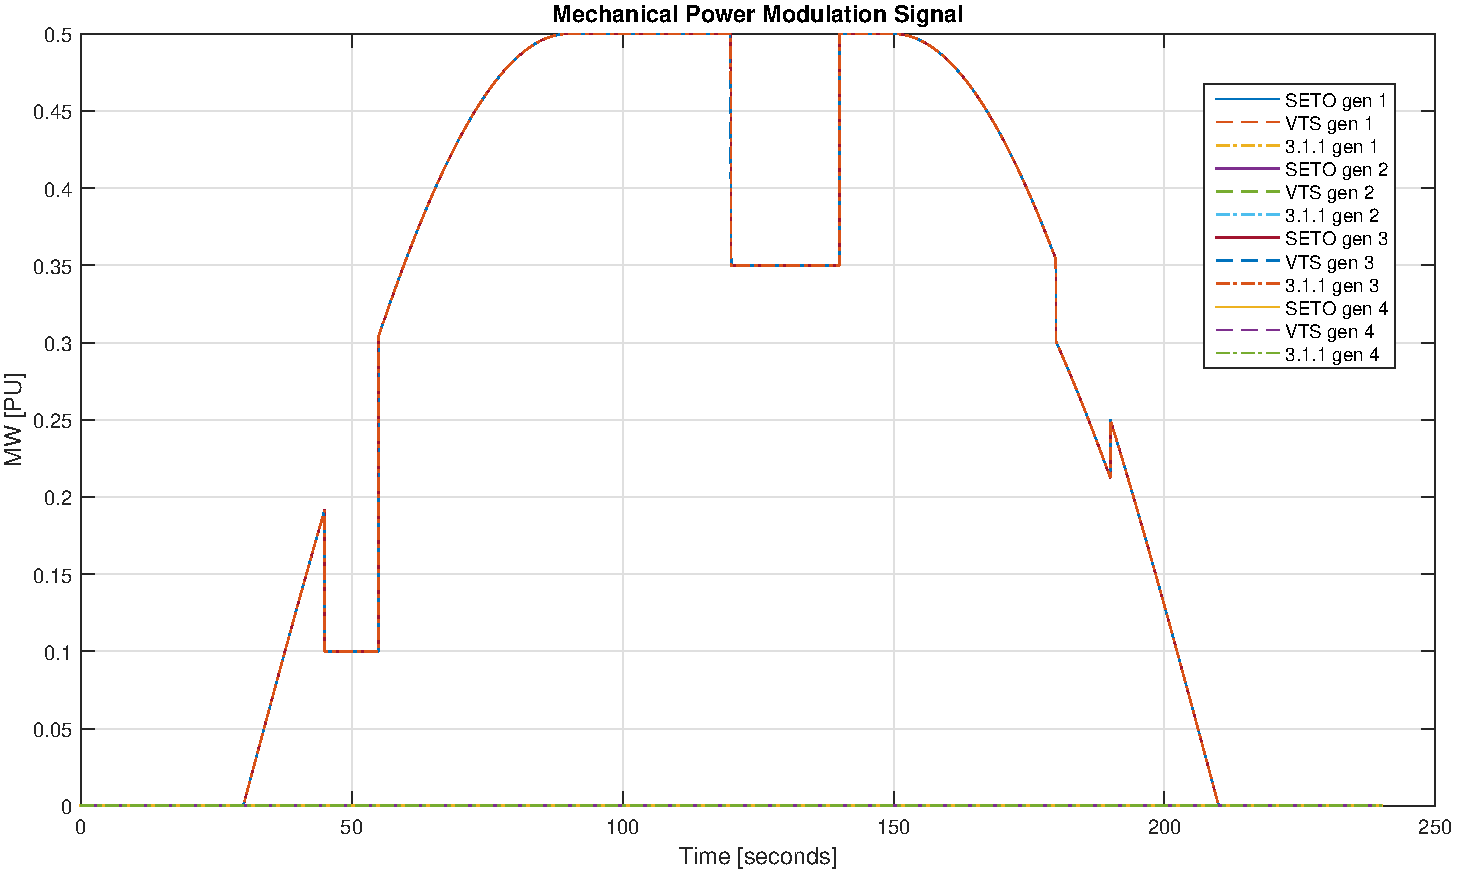
\includegraphics[width=\linewidth]{examples/extendedTerm/verPmSig}
\textbf{Plotted Results - Mechanical Power} \ \\
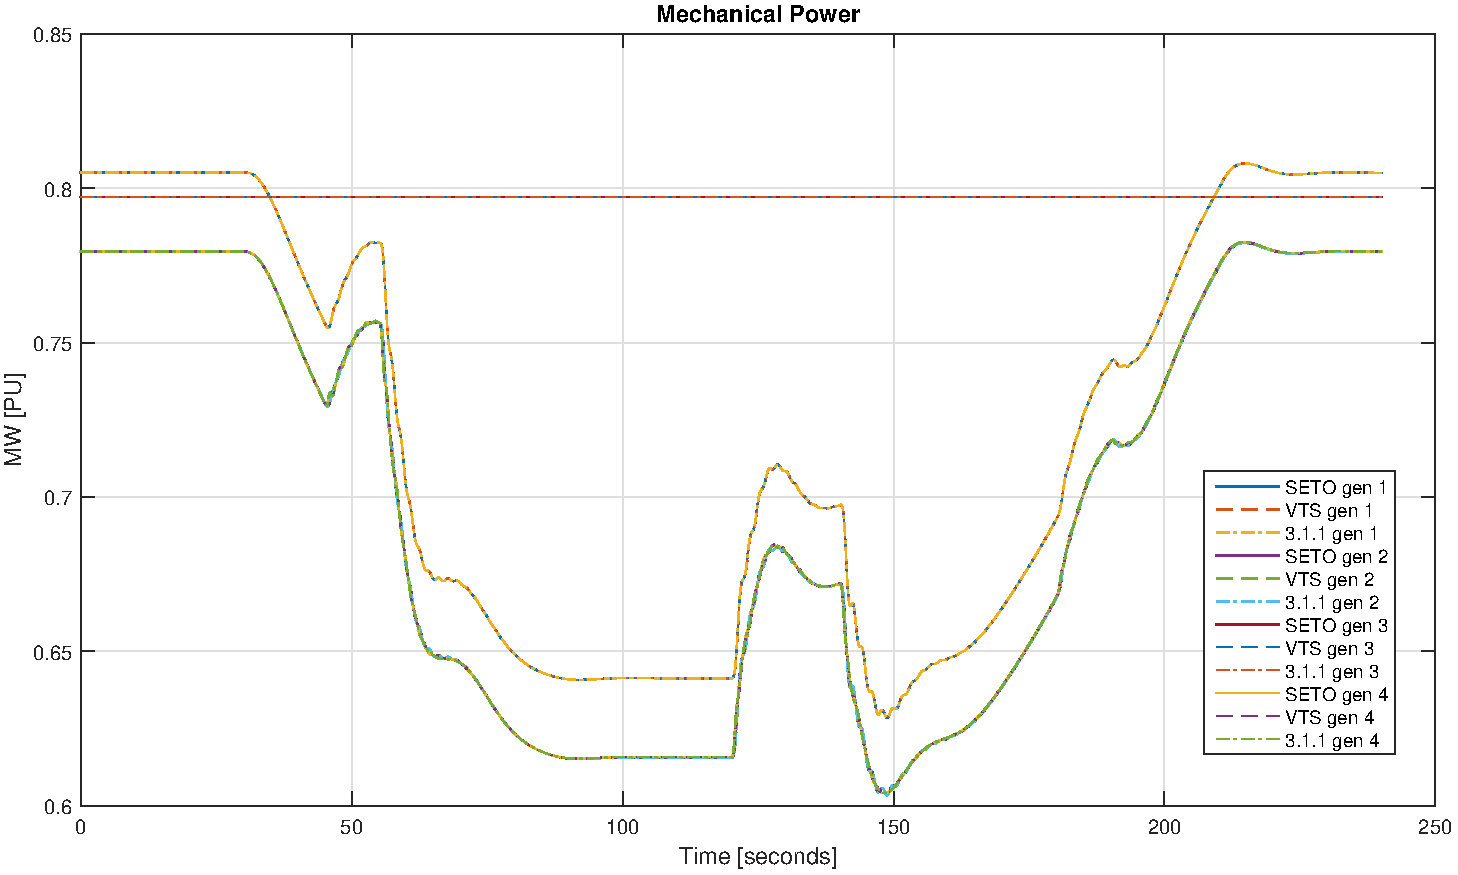
\includegraphics[width=\linewidth]{examples/extendedTerm/verPmech}
Note that the modulated mechanical power signal is not added to the recorded mechanical power.
\textbf{Plotted Results - Electric Power} \ \\
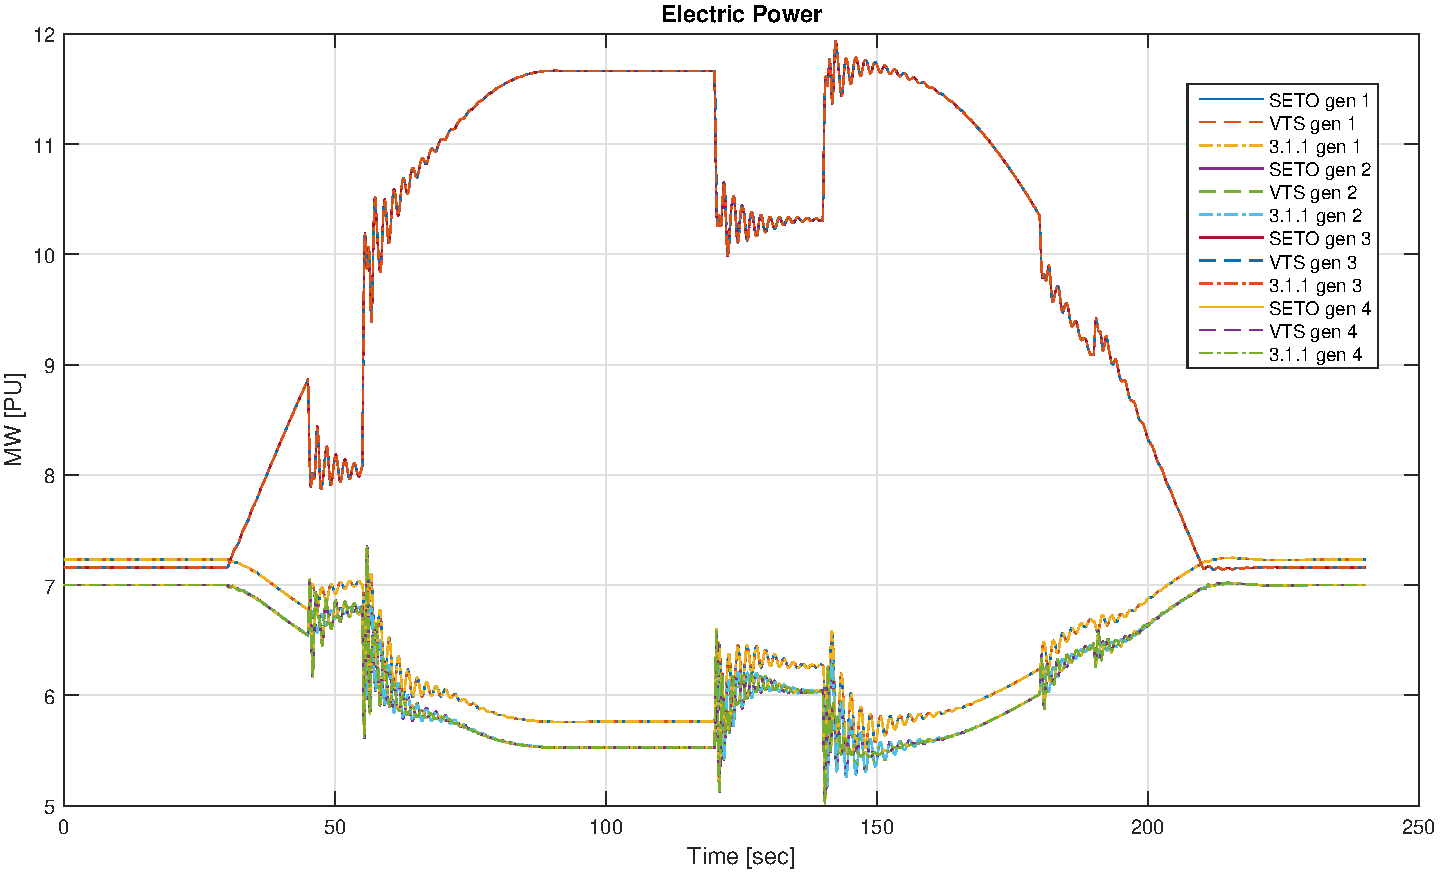
\includegraphics[width=\linewidth]{examples/extendedTerm/verPelect}

\textbf{Plotted Results - Electric Power - Detail} \ \\
Detail of generators 1, 2, and 5 from t= 140 to 150:\\
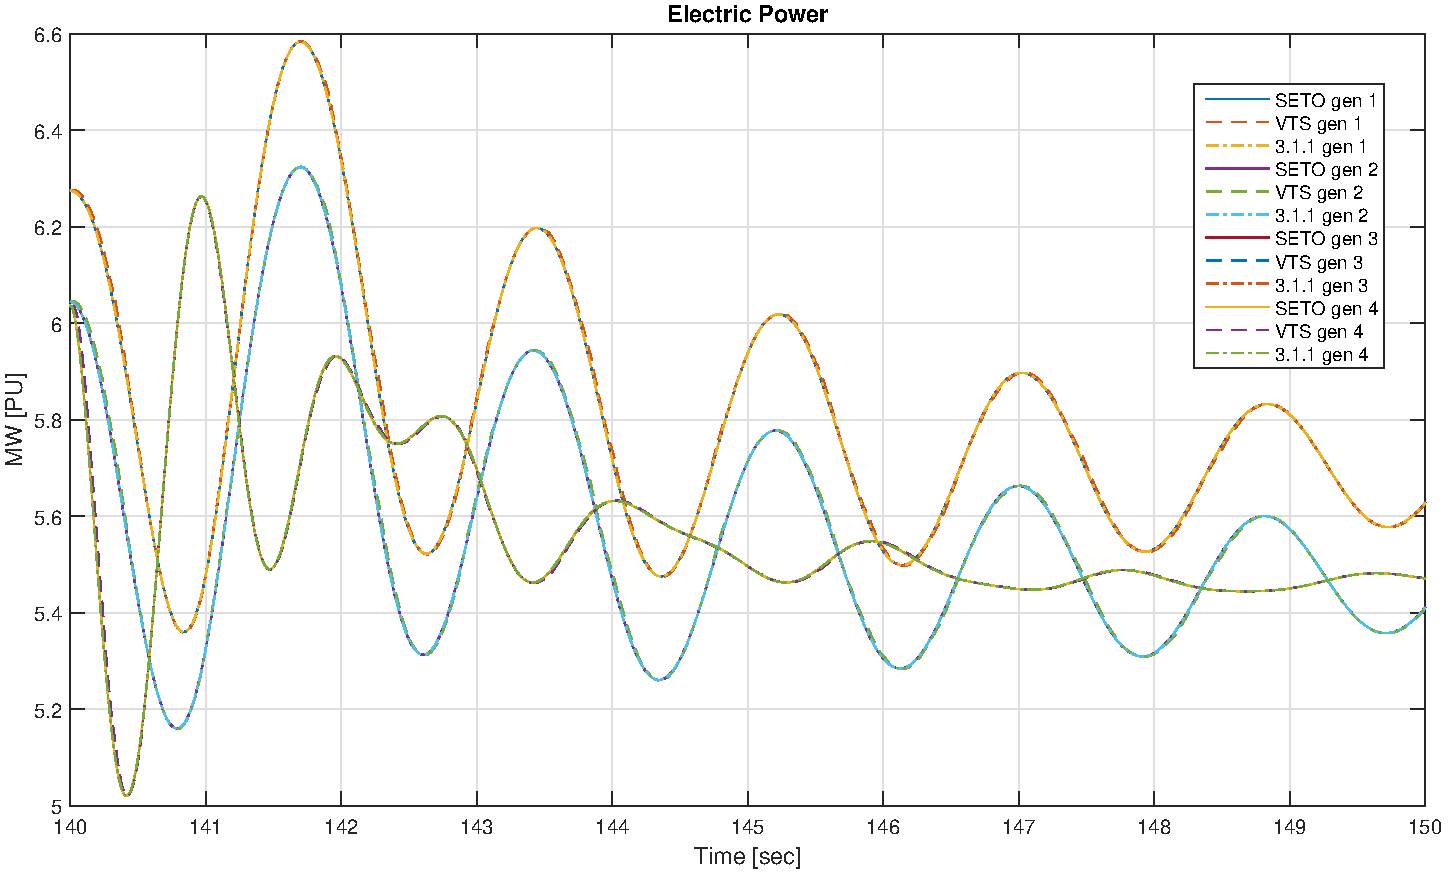
\includegraphics[width=\linewidth]{examples/extendedTerm/verPelectDetail}


%=======================================================================
\pagebreak
\section{ivmmod - WIP} \label{sec: ivmmod ex}
example modified from Dan - includes a VTS example  -
requires some minor reworking - 

shows how angle change `moves' entire system.

VTS method used - clearly shows how variable time steps adjust to capture dynamics


%=======================================================================
\pagebreak
\section{miniWECC - WIP}

	\subsection{AGC - WIP} 
multi area agc (VTS?)

	\subsection{genTrip - WIP} 
use to show arbitrary tripping


%=======================================================================
\pagebreak
\section{pwrmod -WIP} \label{sec: pwrmodExamples}
\subsection{P-injection - WIP}
\subsection{I-injection - WIP}

%=======================================================================
\pagebreak
\section{untrip - WIP}
Sloppily coped from\\ \verb|MT-Tech-SETO\researchDocs\TEX\one-offs\200901-refinedUntripResults2|

Variables to note in associated examples (where \verb|x| is the internal model number):
\begin{itemize}
\item exciter $V_{ref} = $ \verb|g.exc.exc_pot(x,3)|
\item governor $P_{ref} = $ \verb|g.tg.tg_pot(x,5)|
\item governor $\omega_{ref} = $ \verb|g.tg.tg_con(x,3)|
\end{itemize}


\textbf{Test System}\ A simple 3 machine system was used for `un-trip' testing.
All machines were modeled with governors, exciters, and PSS.
Most model parameters are the same, with the exception of MVA base.
Generators 1, 2, and 3, have an $M_{base}$ of 500, 200, and 100 MVA respectively. \\
The experimental goal was to trip Generator 3 off-line, and then `nicely' re-connect it.\\

This is different from the previous test in that ramps of $P_{ref}$ and $\omega_{ref}$ happen concurrently, an extra initialization of the governor was removed, and instead of using \verb|tg_sig| to restore governor $P_{ref}$, the value is ramped directly.

\begin{center}
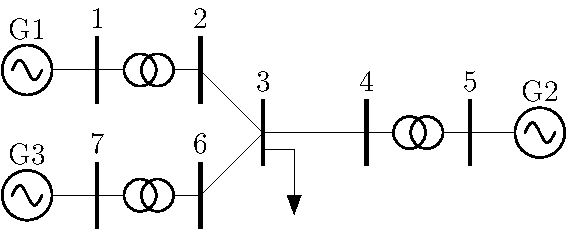
\includegraphics[width=.6\linewidth]{examples/untrip/200831-3mach7bus}
\end{center}

\textbf{Test Event Time Line:}
\begin{itemize}
\itemsep 0 em
\item $t=0$ - System initialized
\item $t=5$ - Generator 3 trips off.
Associated derivatives, $P_{mech}$, and governor $P_{ref}$ set to zero.
\item $t=15$ - Generator 3 re-synced to system and infinite reactance reset to original value. 

\item $t=20-25$ - The governor attached to Generator 3 is reinitialized and the $\omega_{ref}$ value is ramped to its original value. 
This causes mechanical power to be generated by Generator 3 which causes minor transients in system machine speed.
\item $t=35$ - The exciter and PSS on generator 3 is re-initialized and the exciter bypass is removed.
%This causes more reactive power flow into generator 3, the attached bus voltages to decrease, and system speed to increase. 
\item $t=45-65$ - Ramping the governor $P_{ref}$ to the original value increases system speed  and real power flow from Generator 3 while the ramping of exciter reference voltage to its original value decreases system speed and increases reactive power flow from generator 3.
\item $t=150$ - Simulation End
\end{itemize}

\textbf{Observations of Note:}
\begin{itemize}
\itemsep 0 em
%\item The re-connected speed of Generator 3 was set to match Generator 1.
%\item The ramping of R causes a minor 
%\item The exciter was not being initialized to the correct reference voltage time index (i.e. \verb|g.exc.exc_pot(x,3)| referenced index 1 instead of $k$ ). This has been resolved however the exciter still produces a transient when it is bypassed.
\item Nicely `un-tripping' a generator seems possible.
%\item Generator 3 power returns $P_{ref}$ value of 0.5 PU.
\item System appears to return to original state.
%\item Exciter transient caused by bypass removal seems tricky to avoid.\\
%Should probably be reinitialized and enabled at the same time as generator un-trip.
\item Scenario development using FTS as VTS will likely present additional reinitialization issues.
\end{itemize}

\pagebreak
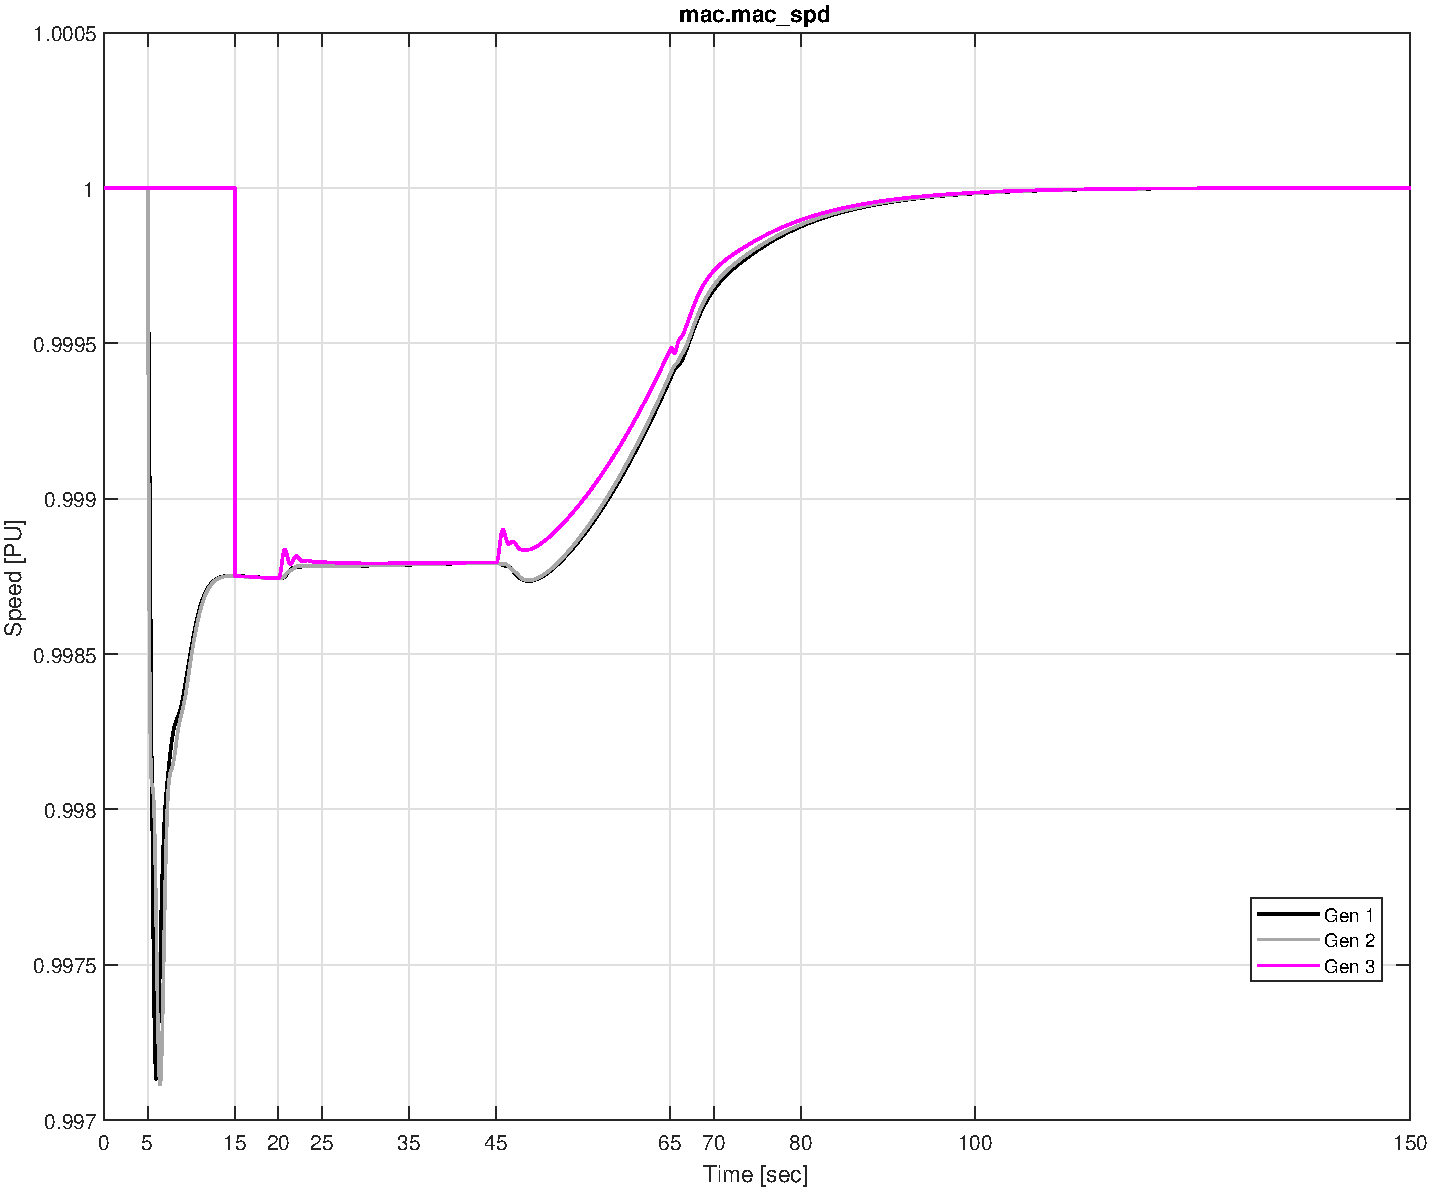
\includegraphics[width=\linewidth]{examples/untrip/combinedSpeed}
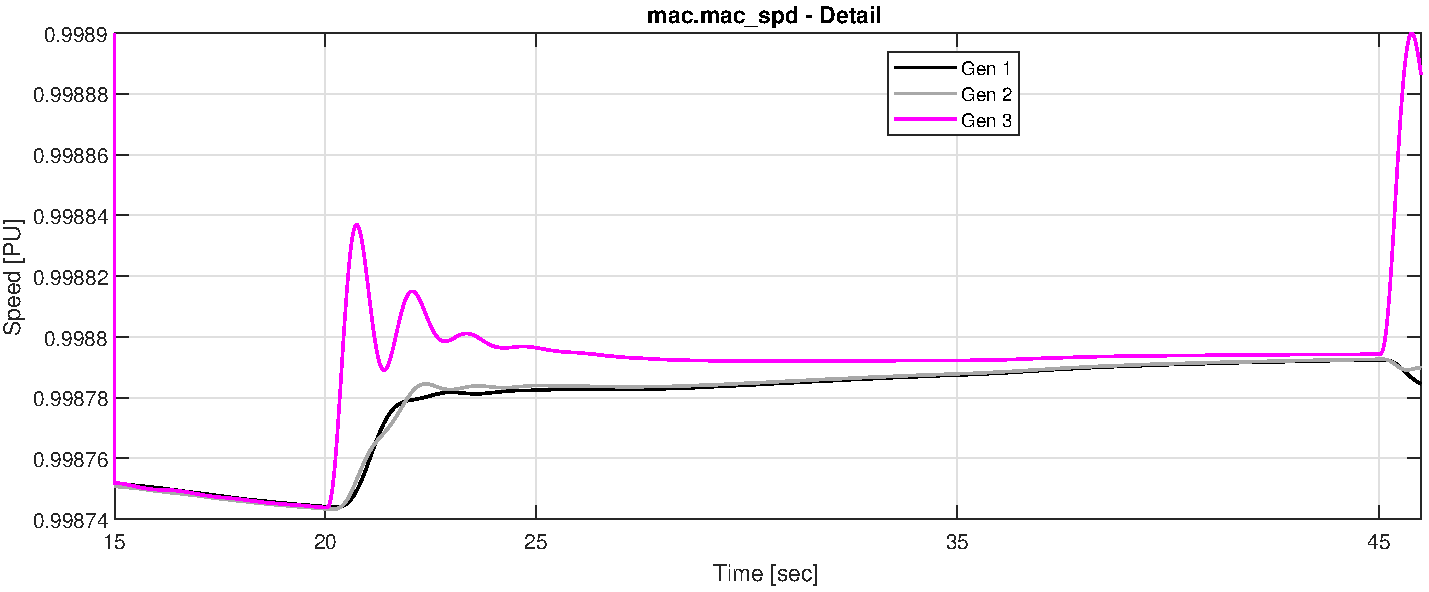
\includegraphics[width=\linewidth]{examples/untrip/combinedSpeedDetail}


\pagebreak
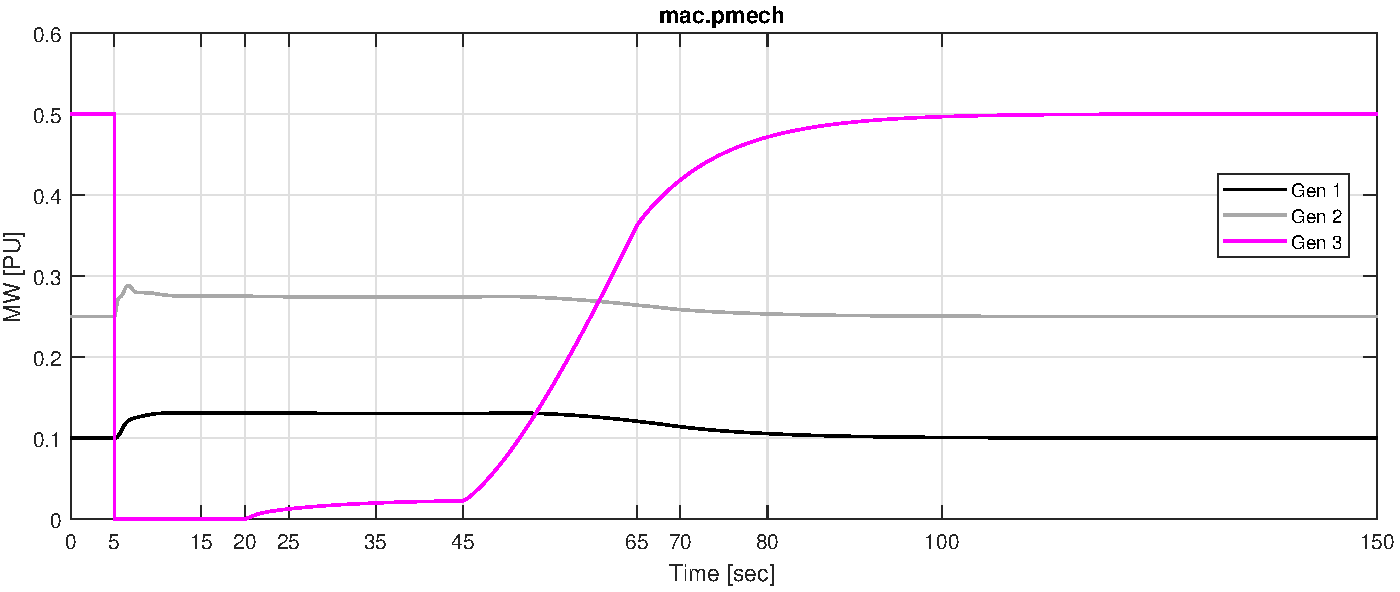
\includegraphics[width=\linewidth]{examples/untrip/combinedPmech}
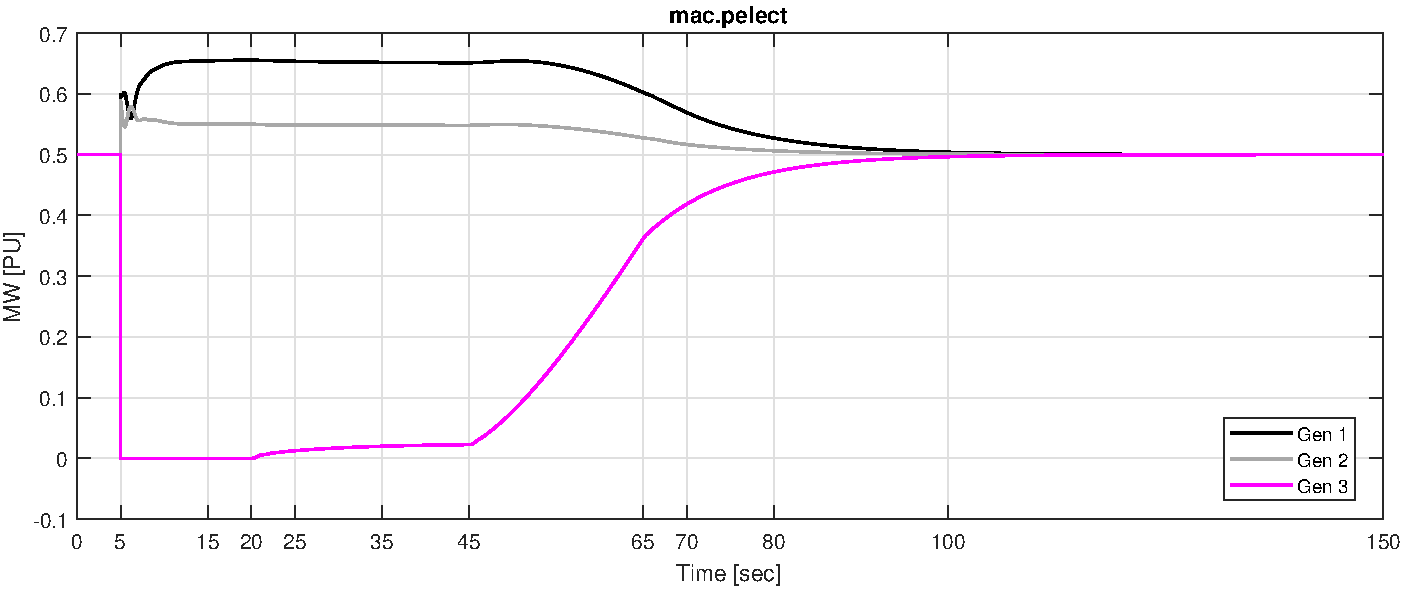
\includegraphics[width=\linewidth]{examples/untrip/combinedPelect}
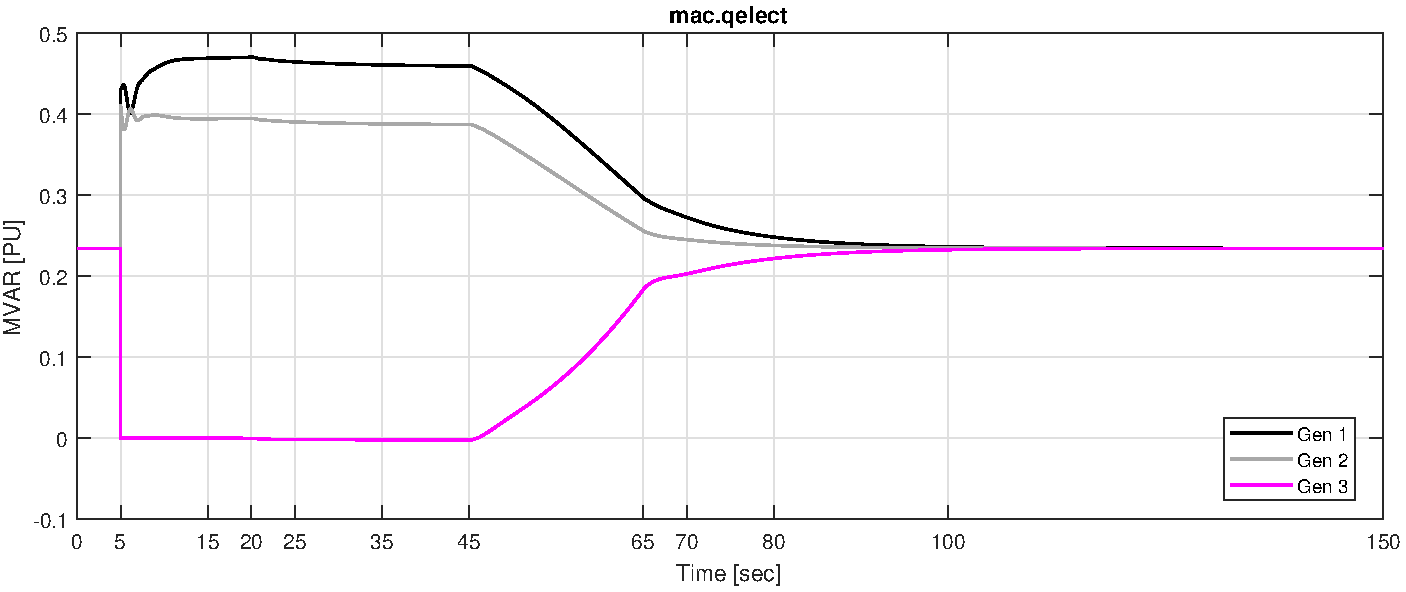
\includegraphics[width=\linewidth]{examples/untrip/combinedQelect}

\pagebreak
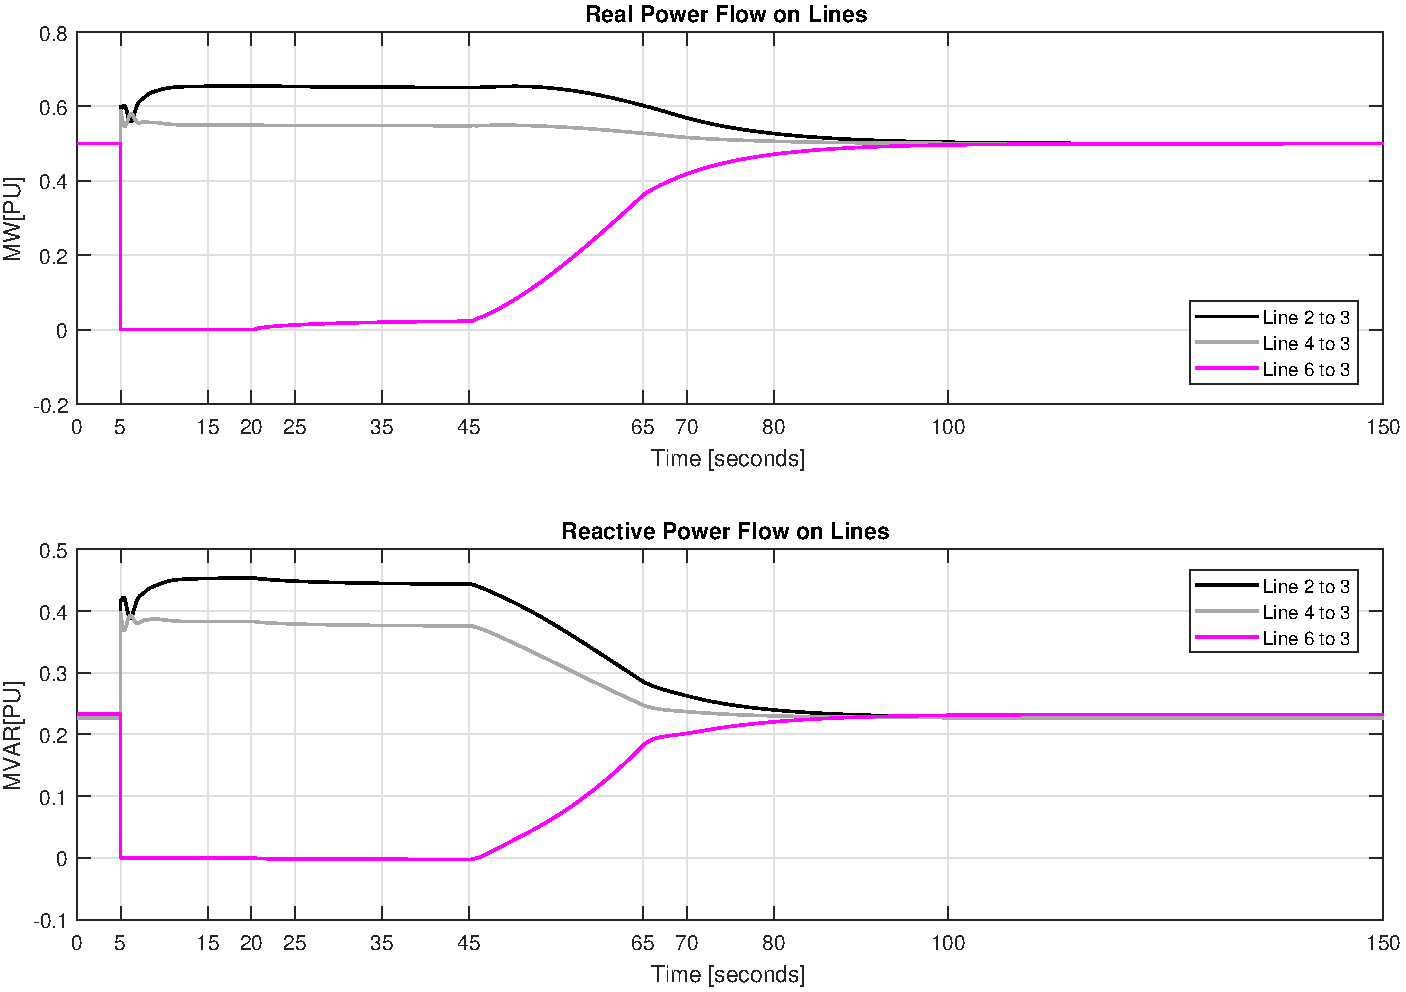
\includegraphics[width=\linewidth]{examples/untrip/combinedLoadFlow}
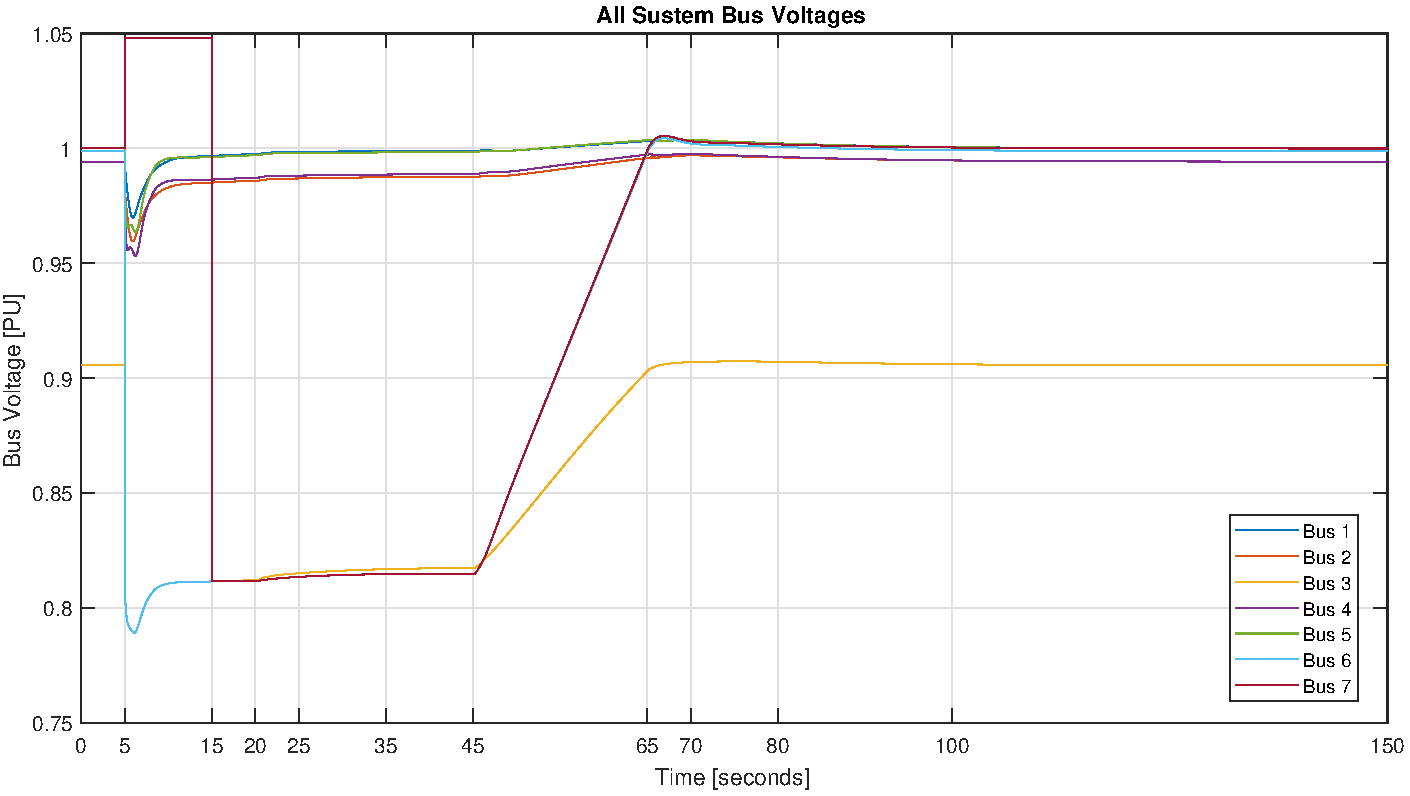
\includegraphics[width=\linewidth]{examples/untrip/combinedBusV}


\pagebreak
\textbf{Machine Trip Logic Code} \ \\
Most `un-trip' action takes place in the \verb|mac_trip_logic| file.
Such actions include:
\begin{itemize}
\item Trip generator 3
\item Set mechanical power to zero and bypass governor
\item Bypass exciter
\item Un-trip generator 3
\item Re-initialize machine
\item Re-init governor
\item Ramp governor $\omega_{ref}$
\item Re-init and remove bypass on exciter and PSS
\item Ramp exciter reference
\end{itemize} 

It should be noted that the \verb|mac_trip_logic| routine usage was created `pre-global g', and as a result, passes variables in and out that are essentially globals.
Realistically, only a data index would need to be passed into the function, and any action can take place directly on the associated \verb|g.mac.mac_trip_states| vector or other required global.

\inputminted[
		frame=lines,
		framesep=2mm,
		baselinestretch=1.2,
		bgcolor=gray!13,
		fontsize=\footnotesize,
		linenos,
		breaklines
		]{MATLAB}% lang
		{../../../../PST/0-examples/unTrip/mac_trip_logic_Gen_3_G2.m}% file name

\pagebreak
\textbf{Turbine Governor Modulation Code} \ \\
The \verb|mtg_sig| file was used to ramp the governors $P_{ref}$ back to the original value.
\inputminted[
		frame=lines,
		framesep=2mm,
		baselinestretch=1.2,
		bgcolor=gray!13,
		fontsize=\footnotesize,
		linenos,
		breaklines
		]{MATLAB}% lang
		{../../../../PST/0-examples/unTrip/mtg_sig_PrefRamp.m}% file name
		
